
\def\problemset#1#2#3{
\noindent\rule{16.5cm}{1pt}
\begin{center}
  \parbox{16.5cm}{\bf
    STAT 598Z Homework 6 \\
    Instructor: Prof. S V N Vishwanathan \hfill Jiajie Huang\\
    Due April 16th, 2013 \hfill huang147@purdue.edu
    }
\end{center}
\noindent\rule{16.5cm}{0.5pt}
}

\newcommand{\lb}[1]{\left \lfloor #1 \right \rfloor}
\newcommand{\bmat}[1]{\begin{bmatrix} #1 \end{bmatrix}}
\documentclass[fleqn, 11pt]{article}
\usepackage{fullpage}
\usepackage{hyperref}
\usepackage{ulem}
\usepackage{amsmath}
\usepackage{algorithm}
%\usepackage{algorithmic}
\usepackage{algpseudocode}
\setlength{\parindent}{0in}
\usepackage{graphics}
\usepackage{graphicx}
\usepackage{mathtools}


\begin{document}

\problemset{3}{Problem Set 2}{\today}


\section*{Problem 1}

\begin{itemize}
\item I used four different initial seeds as means to do the K-Means clustering, as shown in Figure \ref{F01} and \ref{F02}. And I used square, triangle and sphere to represent data points from the 3 Gaussian distributions, respectively. We can see that the distribution of clustering results are similar in all four situations. The change of $J(r,u)$ is shown in Figure \ref{F1}. We can see that $J(r,u)$ of different initial seeds all converged to the same value, except for a minor difference in the converging rate. 

\begin{figure}[htb]
\centering
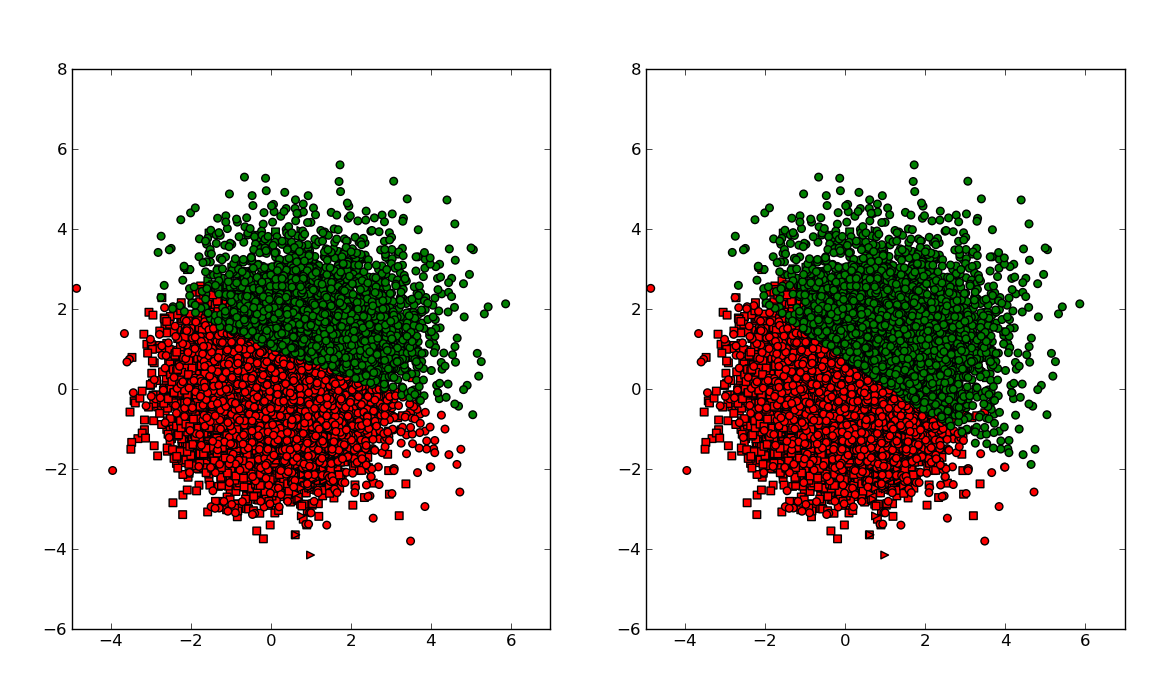
\includegraphics[width=18cm]{F01.png}
\caption{Visualization of K-Means Clustering Using Two Different Initial Seeds ($K=2$)}
\label{F01}
\end{figure}

\begin{figure}[htb]
\centering
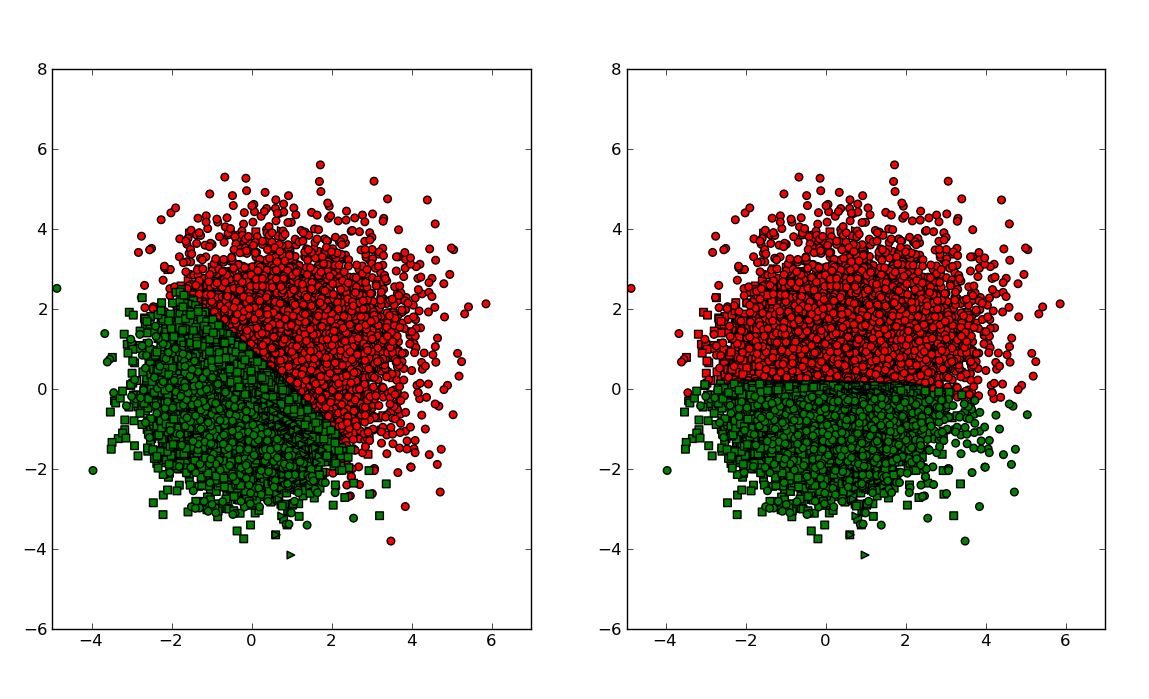
\includegraphics[width=18cm]{F02.png}
\caption{Visualization of K-Means Clustering Using Two Other Different Initial Seeds ($K=2$)}
\label{F02}
\end{figure}

\begin{figure}[htb]
\centering
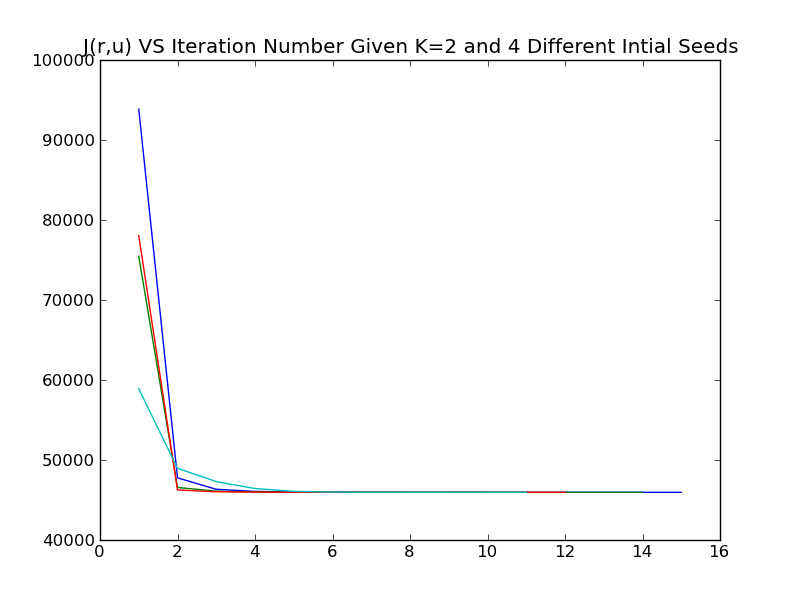
\includegraphics[width=15cm]{F1.png}
\caption{$J(r,u)$ v.s. Iteration Numbers}
\label{F1}
\end{figure}


\item I keep the initial seed the same, but change the value of $k$ to be $2,3,...,6$. The visualization of clustering and change of $J(r,u)$ are shown in Figures \ref{F21}, \ref{F22} and \ref{F3}. The value of $J(r,u)$ (Figure \ref{F3}) gets lower as Iteration Number increases; the minimum values of $J(r,u)$ also decreases as $K$ increases: for $K=2,3,4,5,6$ $J(r,u)$ are $236$,$190$,$150$,$117$, and $107$ (rounded). So when $K=6$ the value of $J(r,u)$ gets the lowest. The distributions of clustering also differ a lot with different $K$ values. To figure out the best $K$ value, I also calculated the purity in each cluster, which is the maximum percentage of points from the same Gaussian distribution. The larger the purity, the more similar the points are in the cluster, so the better clustering it is. Looking through $K=2,...,6$, we want a clustering that has relatively high purity in each cluster and also has a relatively low $J(r,u)$. Balancing both characteristics, I think $K=4$ does the best job. It has a $J(r,u)=150$, for away from the maximum $J(r,u)=236$, and not far away from the minimum $J(r,u)=107$. And the purity when $K=4$ is $[0.91176470588235292, 0.7857142857142857, 0.88888888888888884, 0.55172413793103448]$, which is relatively high for all clusters, comparing to other clustering methods.

\begin{verbatim}
K=2,3,4,5,6!!

K: 2 Seed: 30
Iteration: 1  J(r,u): 349.389115369
Iteration: 2  J(r,u): 262.695090655
Iteration: 3  J(r,u): 250.745103117
Iteration: 4  J(r,u): 247.601074241
Iteration: 5  J(r,u): 240.7570529
Iteration: 6  J(r,u): 236.19315226
Purities in 2 classes: 
[0.77966101694915257, 0.58536585365853655]

K: 3 Seed: 30
Iteration: 1  J(r,u): 255.748828223
Iteration: 2  J(r,u): 191.034795635
Iteration: 3  J(r,u): 190.611716202
Iteration: 4  J(r,u): 190.238116299
Purities in 3 classes: 
[0.5, 0.86956521739130432, 0.65625]

K: 4 Seed: 30
Iteration: 1  J(r,u): 220.464413702
Iteration: 2  J(r,u): 154.392972069
Iteration: 3  J(r,u): 150.385259237
Purities in 4 classes: 
[0.91176470588235292, 0.7857142857142857, 0.88888888888888884, 0.55172413793103448]

K: 5 Seed: 30
Iteration: 1  J(r,u): 196.781801235
Iteration: 2  J(r,u): 129.736789092
Iteration: 3  J(r,u): 119.810794795
Iteration: 4  J(r,u): 116.849929349
Purities in 5 classes: 
[0.84615384615384615, 0.77777777777777779, 0.48148148148148145, 0.967741935483871, 0.5714285714285714]

K: 6 Seed: 30
Iteration: 1  J(r,u): 213.616799381
Iteration: 2  J(r,u): 115.70384947
Iteration: 3  J(r,u): 107.418080073
Purities in 6 classes: 
[1.0, 0.8125, 1.0, 0.5714285714285714, 0.83870967741935487, 0.47826086956521741]

\end{verbatim}

\begin{figure}[htb]
\centering
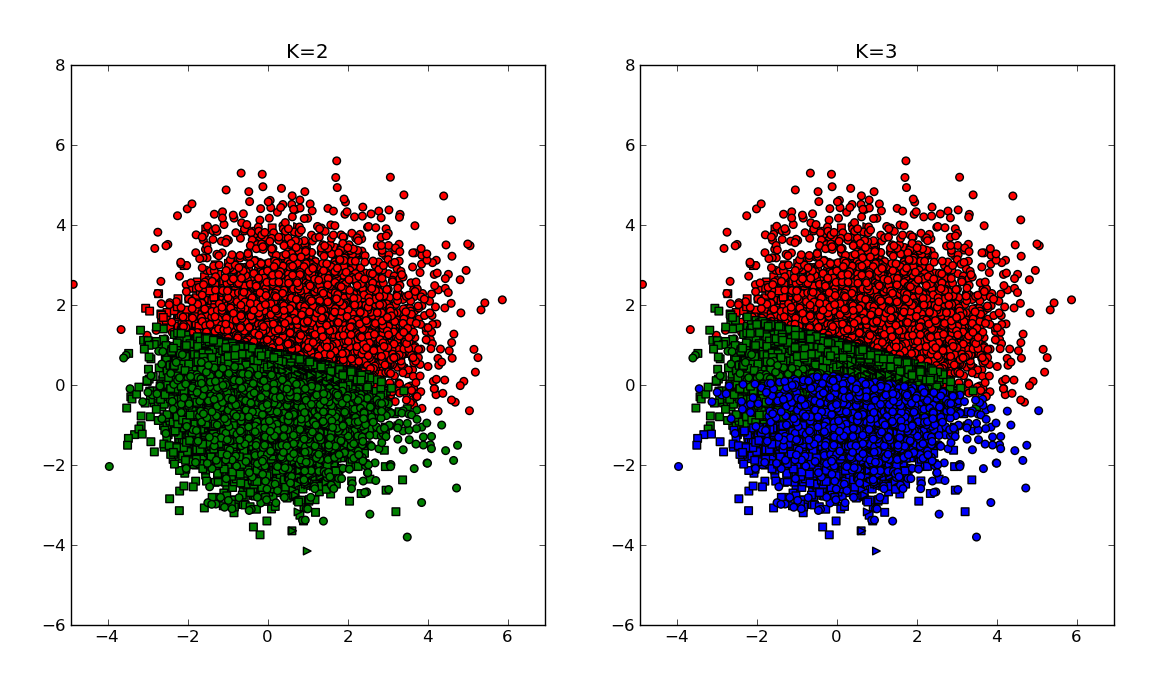
\includegraphics[width=12cm]{F21.png}
\caption{Visualization of K-Means Clustering Using $K=2,3$}
\label{F21}
\end{figure}

\begin{figure}[htb]
\centering
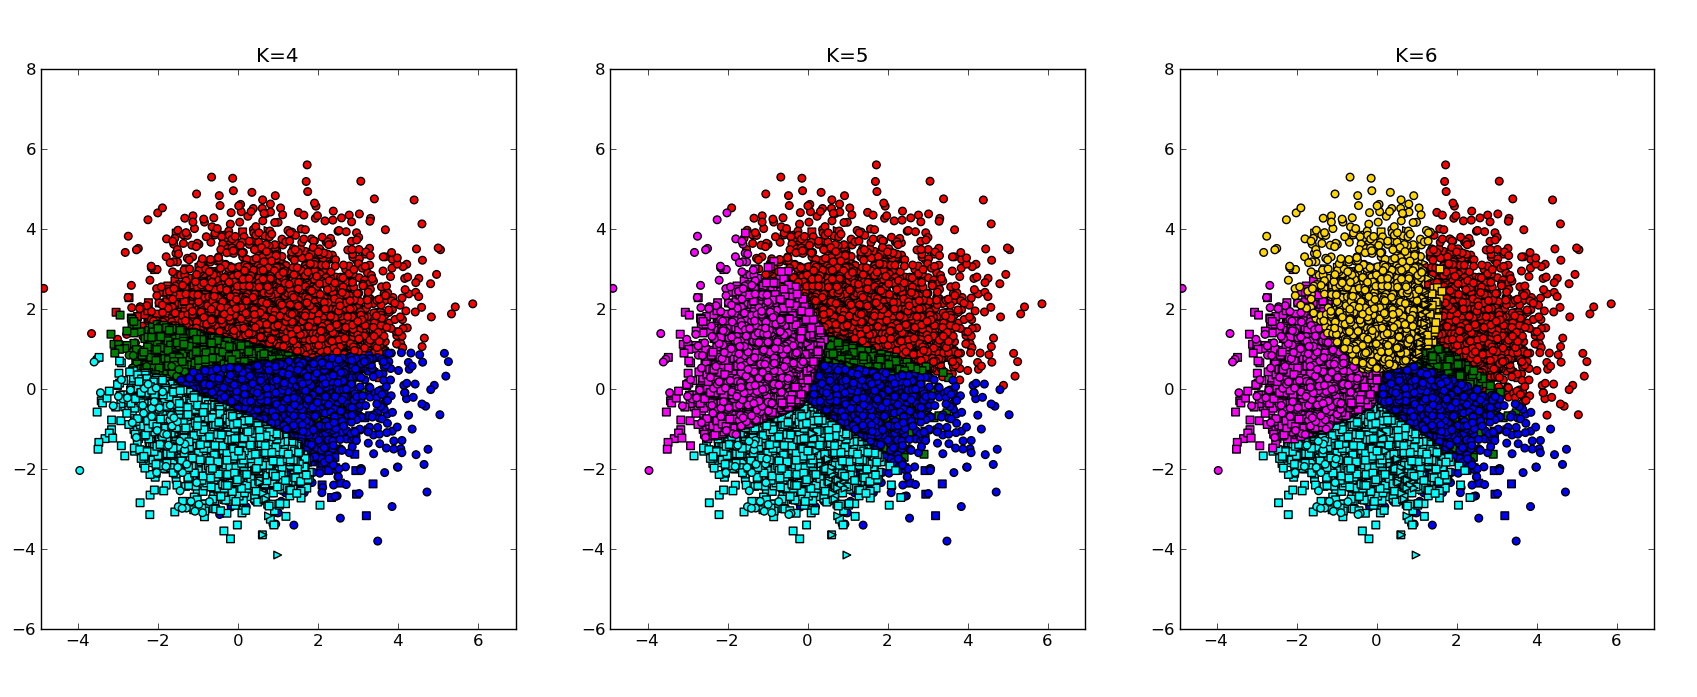
\includegraphics[width=18cm]{F22.png}
\caption{Visualization of K-Means Clustering Using $K=4,5,6$}
\label{F22}
\end{figure}

\begin{figure}[htb]
\centering
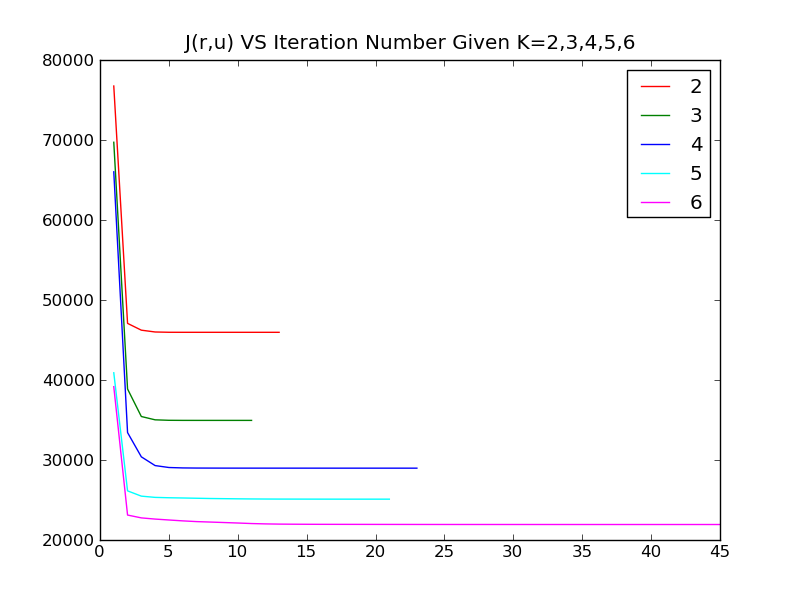
\includegraphics[width=15cm]{F3.png}
\caption{$J(r,u)$ v.s. Iteration Numbers}
\label{F3}
\end{figure}
 

\item I kept $K=3$ and used $10$ different random initial seeds to test on the distribution of clustering. The visualization of clustering is shown in Figure \ref{F41}, \ref{F42}, \ref{F43}, \ref{F44}, and \ref{F45}. The change of $J(r,u)$ is shown in Figure \ref{F5}. We can easily see that the $10$ different random seeds have similar results in both the clustering distribution, and the minimization of distances ($J(r,u)$). 

\begin{figure}[htb]
\centering
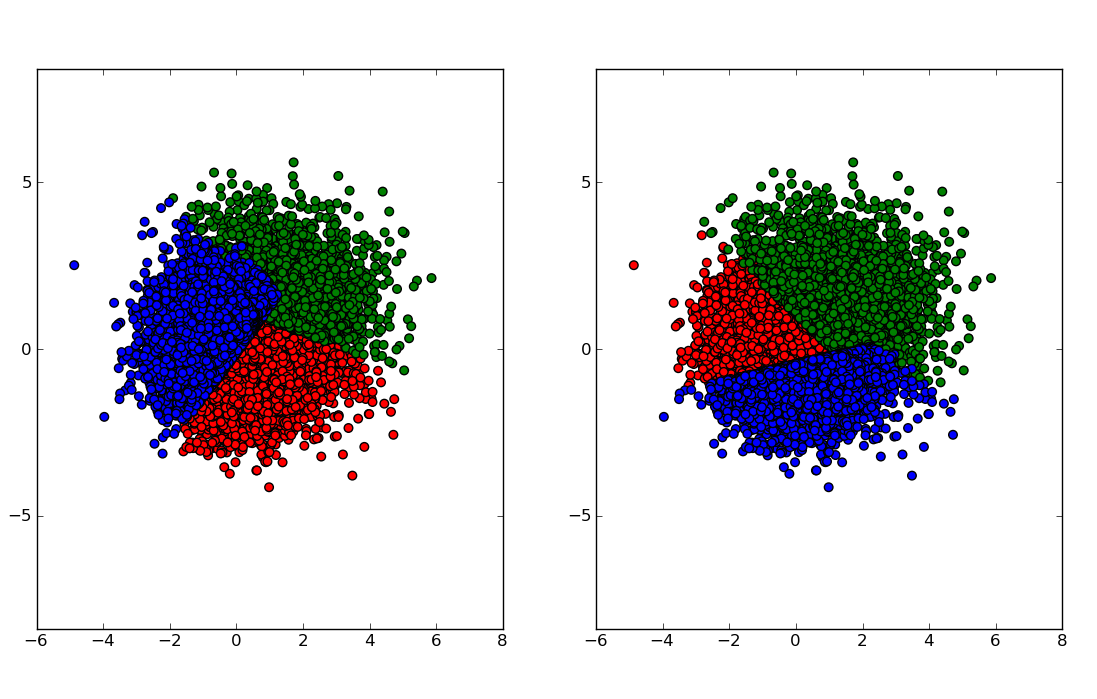
\includegraphics[width=12cm]{F41.png}
\caption{Visualization of K-Means Clustering Using Two Different Initial Seeds ($K=3$)}
\label{F41}
\end{figure}

\begin{figure}[htb]
\centering
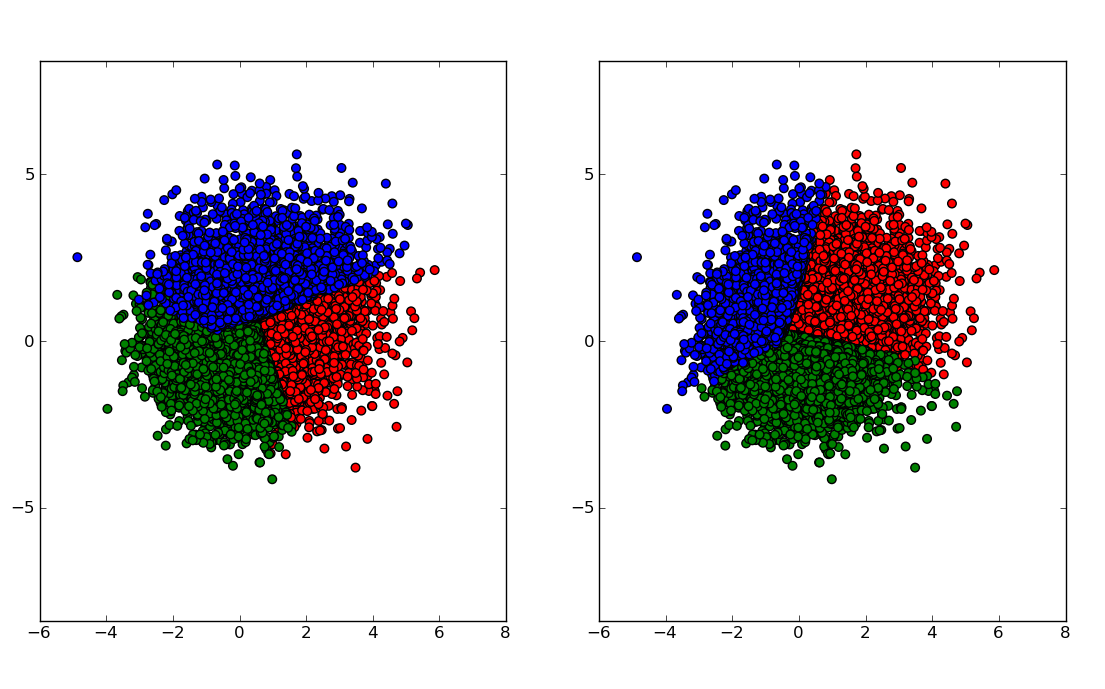
\includegraphics[width=12cm]{F42.png}
\caption{Visualization of K-Means Clustering Using Two Other Different Initial Seeds ($K=3$)}
\label{F42}
\end{figure}

\begin{figure}[htb]
\centering
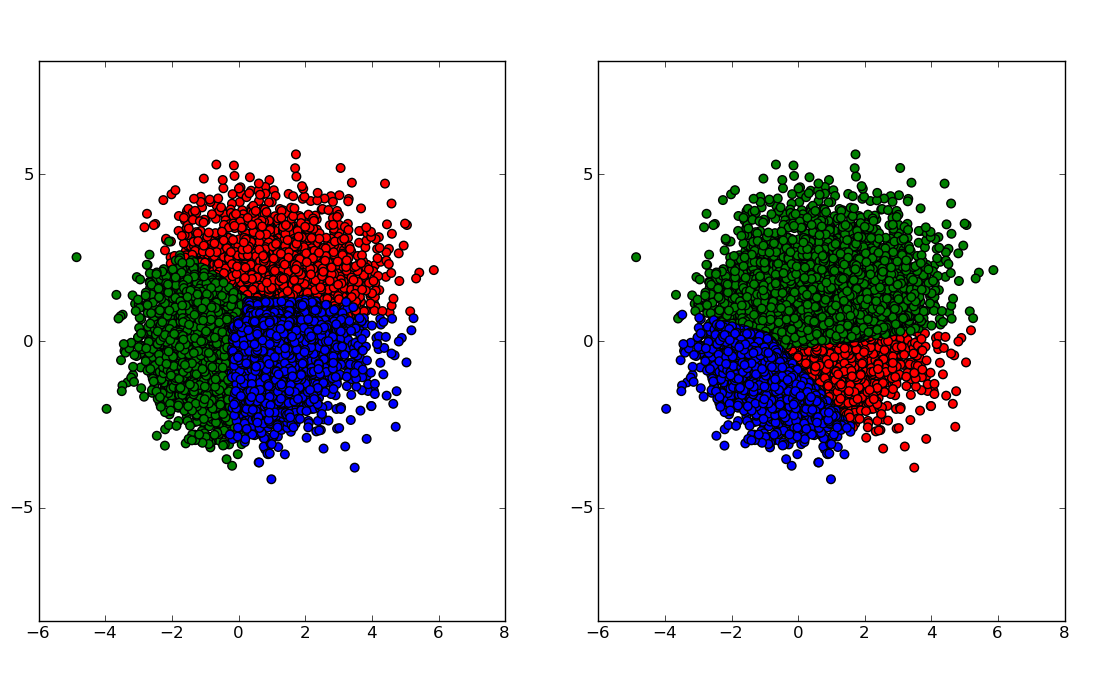
\includegraphics[width=12cm]{F43.png}
\caption{Visualization of K-Means Clustering Using Two Other Different Initial Seeds ($K=3$)}
\label{F43}
\end{figure}

\begin{figure}[htb]
\centering
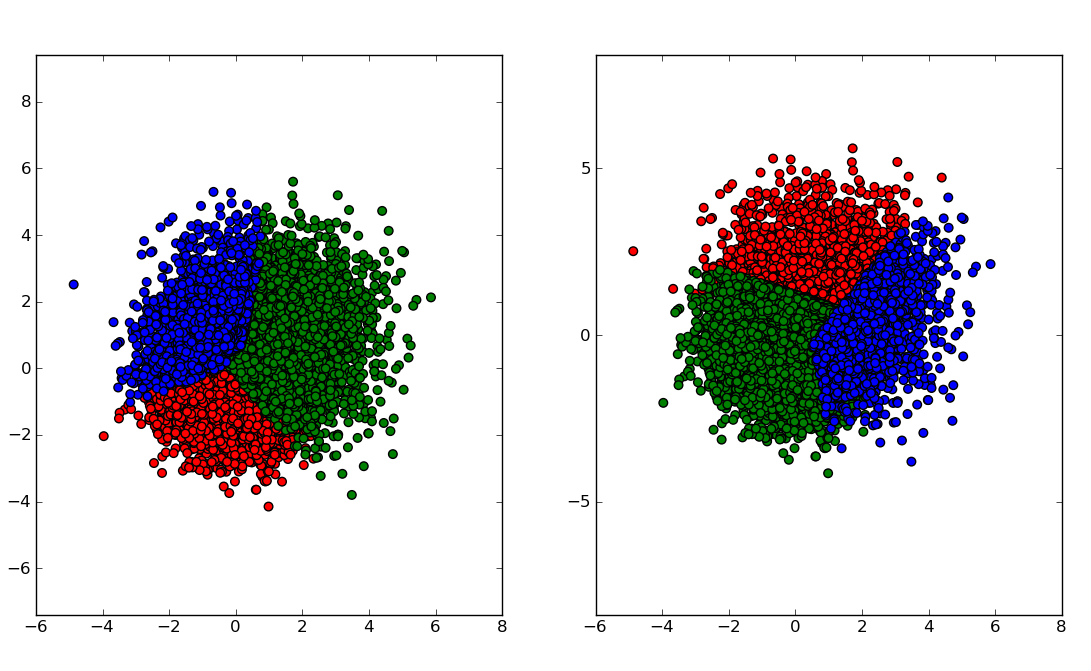
\includegraphics[width=12cm]{F44.png}
\caption{Visualization of K-Means Clustering Using Two Other Different Initial Seeds ($K=3$)}
\label{F44}
\end{figure}

\begin{figure}[htb]
\centering
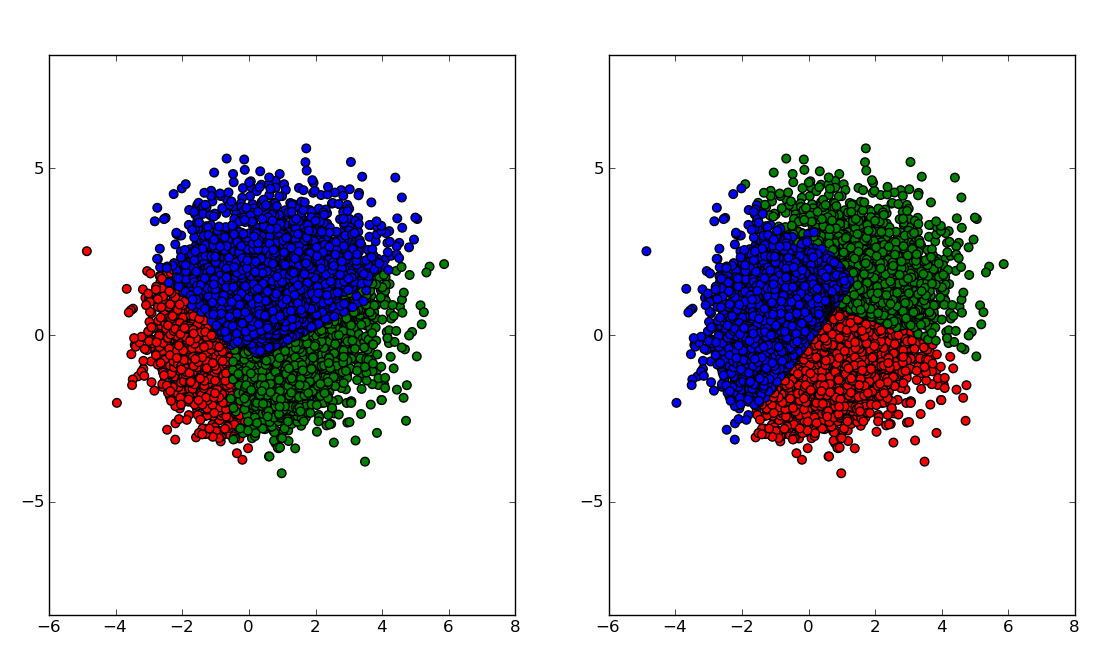
\includegraphics[width=12cm]{F45.png}
\caption{Visualization of K-Means Clustering Using Two Other Different Initial Seeds ($K=3$)}
\label{F45}
\end{figure}

\begin{figure}[htb]
\centering
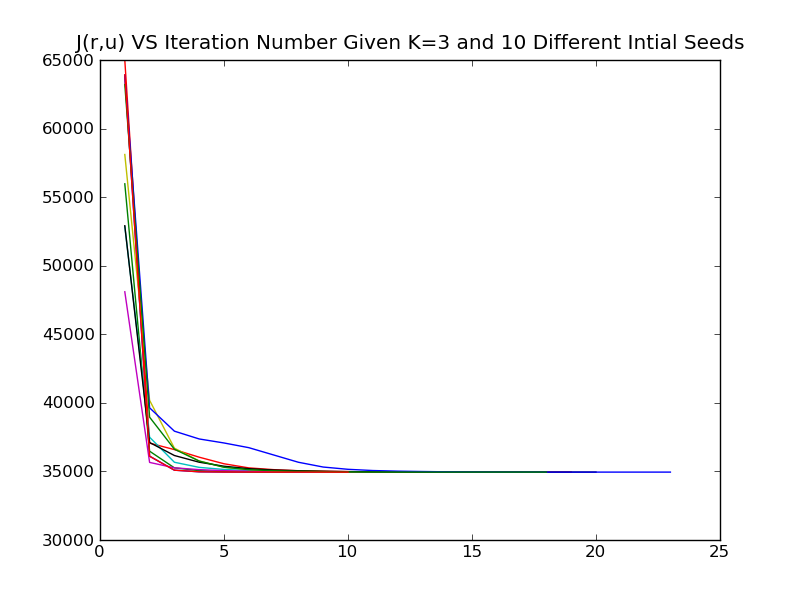
\includegraphics[width=15cm]{F5.png}
\caption{$J(r,u)$ v.s. Iteration Numbers}
\label{F5}
\end{figure}


\item I kept $K=3$ and the same initial seed, but changed the mean values of the $3$ Gaussian distributions from $[0,0],[1,0],[1,1]$ to $[-1, 0],[1, 0],[0, 1]$(Spread-out) and $[0, 0],[0, 0.5],[0, 1]$(Close-up). The purity of each clustering are shown below, we learn that the more close-up the points are, the lower purity the clustering is. So the Spread-out points have the highest purity and thus best in separation. The clustering visualization is shown in Figure \ref{F6}. When looking at the change of $J(r,u)$ in Figure \ref{F7}, we find that the more close-up the points are, the easier to find a convergence of $J(r,u)$, and the value of $J(r,u)$ is also low. That tells us that we can not only determine the quality of clustering based on the value and convergence of $J(r,u)$ but we need to also look at the purity. 


\begin{verbatim}
3 Different Mean Values Given K=3!!

Original Means
Mean1: [0, 0] Mean2: [1, 0] Mean3: [0, 1]
K: 3 Seed: 30
...
Iteration: 34  J(r,u): 35512.468781
Purities in 3 classes: 
[0.49061196105702365, 0.9263759828448892, 0.584287317620651]

Spread-out Means
Mean1: [-1, 0] Mean2: [1, 0] Mean3: [0, 1]
K: 3 Seed: 30
...
Iteration: 35  J(r,u): 36632.0234786
Purities in 3 classes: 
[0.45540075990591639, 0.966066229985444, 0.41855788566503876]

Close-up Means
Mean1: [0, 0] Mean2: [0, 0.5] Mean3: [0, 1]
K: 3 Seed: 30
...
Iteration: 22  J(r,u): 35143.2752124
Purities in 3 classes: 
[0.42643391521197005, 0.91406617531754741, 0.73117742539642905]
\end{verbatim}

\begin{figure}[htb]
\centering
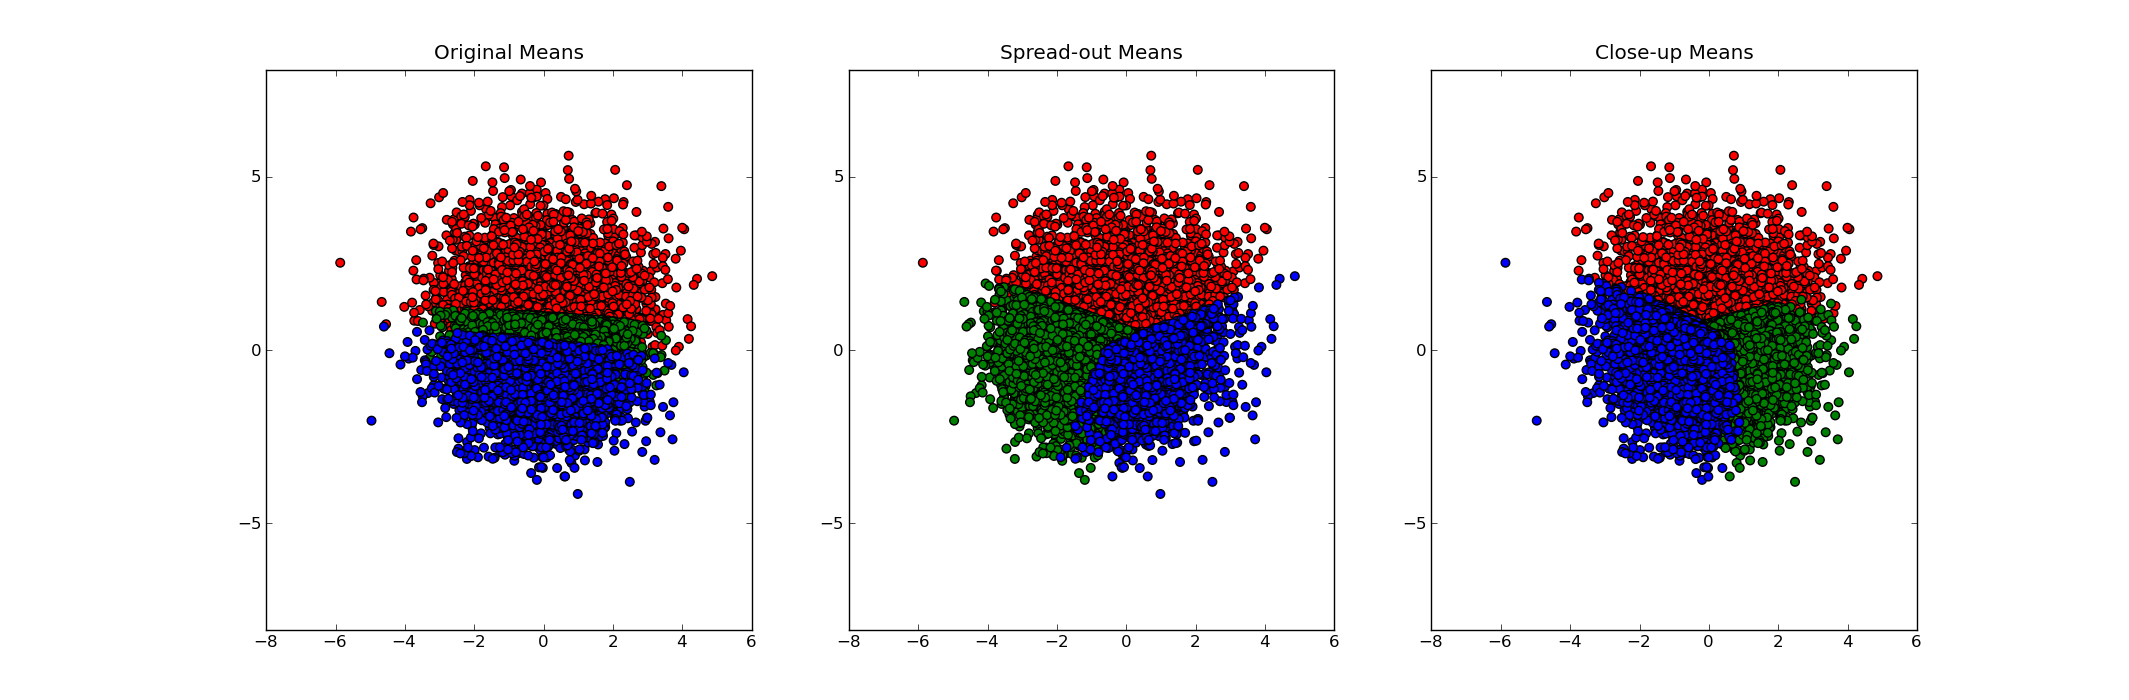
\includegraphics[width=18cm]{F6.png}
\caption{Visualization of K-Means Clustering Using Three Different Mean Values ($K=3$)}
\label{F6}
\end{figure}

\begin{figure}[htb]
\centering
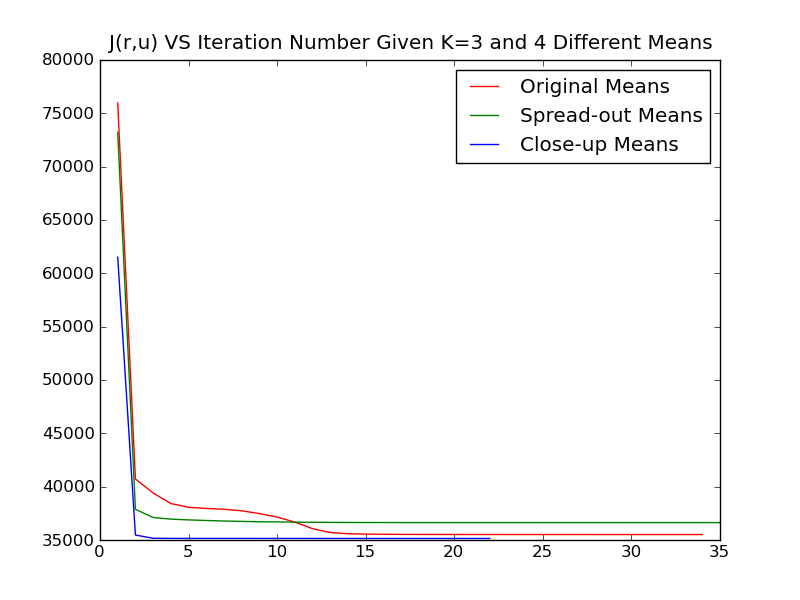
\includegraphics[width=15cm]{F7.png}
\caption{$J(r,u)$ v.s. Iteration Numbers}
\label{F7}
\end{figure}


\item I kept $K=3$ and the same initial seed, but changed the variance values of the $3$ Gaussian distributions from 
\[[[1, 0], [0, 1]], [[0.1, 0], [0, 1]],[[2, 0], [0, 2]]\] 
to (Small Variance) 
\[[[0.1, 0], [0, 0.1]],[[0.01, 0], [0, 0.1]],[[0.2, 0], [0, 0.2]]\]
and (Large Variance)
\[[[3, 0], [0, 3]],[[0.3, 0], [0, 3]],[[6, 0], [0, 6]]\]
. 
Obviously, when the variance is small, the points are close-up to the center of each Gaussian distribution, thus K-Means clustering has a better separation in the points, so the purity for small variance is the best. We can also look at the Small Variance subplot in Figure \ref{F9}, which shows that most of the points are clustered into the center shown in blue, and that agrees with the original model that $70\%$ of points comes from the center (mean is $[0,0]$) Gaussian distribution. A small variance also helps in the convergence in $J(r,u)$ and has a lower $J(r,u)$ value as shown in Figure \ref{F9}. 

\begin{verbatim}
3 Different Variances Given K=3!!

Var1: [[1, 0], [0, 1]] Var2: [[0.1, 0], [0, 1]] Var3: [[2, 0], [0, 2]]

K: 3 Seed: 30
...
Iteration: 34  J(r,u): 35512.468781
Purities in 3 classes: 
[0.49061196105702365, 0.9263759828448892, 0.584287317620651]

Var1: [[0.1, 0], [0, 0.1]] Var2: [[0.01, 0], [0, 0.1]] Var3: [[0.2, 0], [0, 0.2]]

K: 3 Seed: 30
...
Iteration: 9  J(r,u): 4624.61488682
Purities in 3 classes: 
[0.74108527131782942, 0.99985211475894709, 0.65734865374721319]

Var1: [[3, 0], [0, 3]] Var2: [[0.3, 0], [0, 3]] Var3: [[6, 0], [0, 6]]

K: 3 Seed: 30
...
Iteration: 48  J(r,u): 80763.949289
Purities in 3 classes: 
[0.55916386711459498, 0.74062278839348905, 0.7665476963011032]
\end{verbatim}

\begin{figure}[htb]
\centering
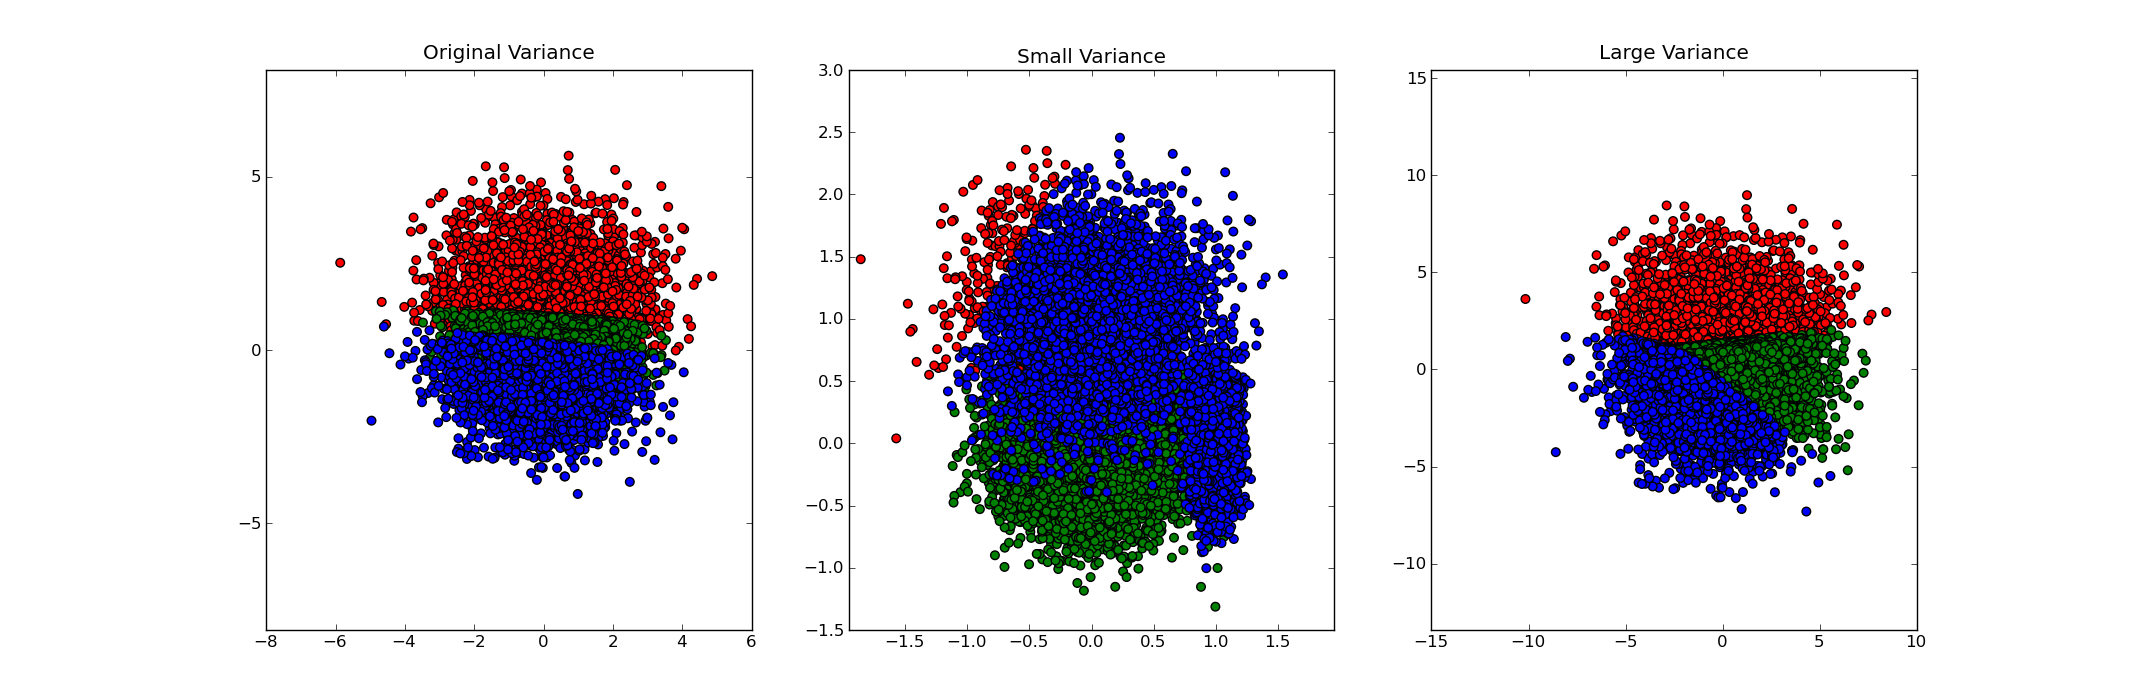
\includegraphics[width=18cm]{F8.png}
\caption{Visualization of K-Means Clustering Using Three Different Variance Values ($K=3$)}
\label{F8}
\end{figure}

\begin{figure}[htb]
\centering
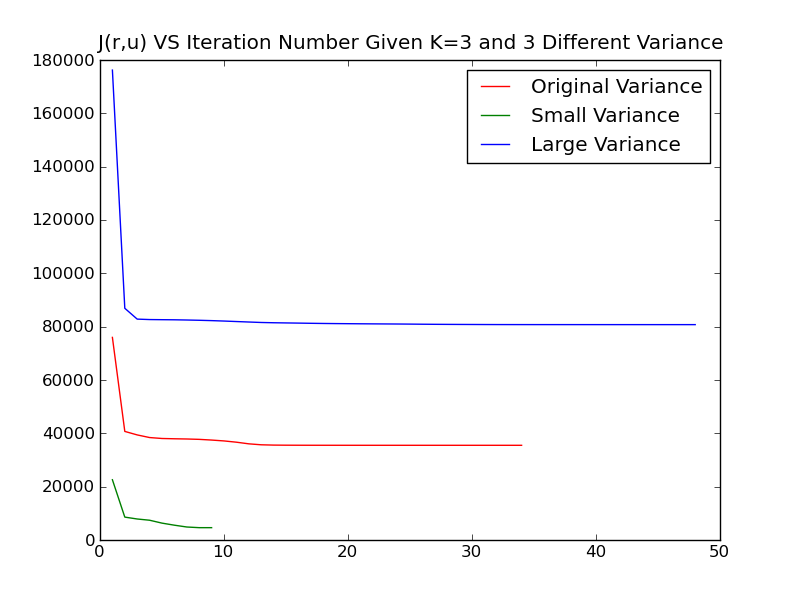
\includegraphics[width=15cm]{F9.png}
\caption{$J(r,u)$ v.s. Iteration Numbers}
\label{F9}
\end{figure}


\item I wrote a program for the Gaussian Mixture Model and the results of clustering assignments are shown in Figures \ref{gmm}; The distribution of each cluster in $X$ and $Y$ dimensions are shown in \ref{gmmhist}, respectively. For visualization I set the points to be clustered into the Gaussian distribution with highest $\gamma$ value. I set the maximum iteration to be $10000$, and the tolerance of difference in $\gamma$ as $0.001$. The value of difference finally converged in $17$ iterations. 

\begin{verbatim}
diff 1.0
diff 0.247866014954
diff 0.0311447554769
diff 0.0239822131299
diff 0.0209311785987
diff 0.0174222991875
diff 0.0140759698151
diff 0.0111796108491
diff 0.00878255676385
diff 0.00684495360007
diff 0.00530996310052
diff 0.0041120766978
diff 0.00318604679511
diff 0.00247052366001
diff 0.00192263148965
diff 0.00150724858789
diff 0.00119614961777
converged in 17 iterations
\end{verbatim}


\begin{figure}[htb]
\centering
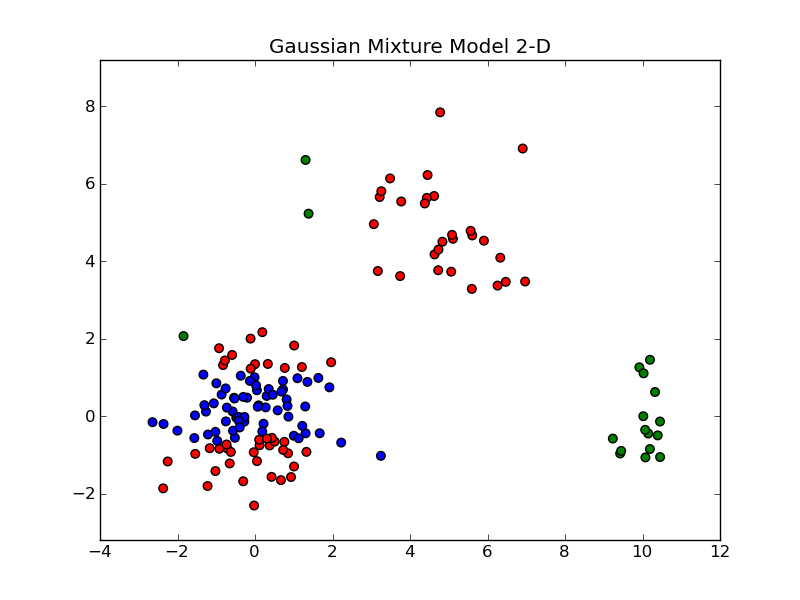
\includegraphics[width=18cm]{GMM.png}
\caption{Visualization of Gaussian Mixture Model}
\label{gmm}
\end{figure}

\begin{figure}[htb]
\centering
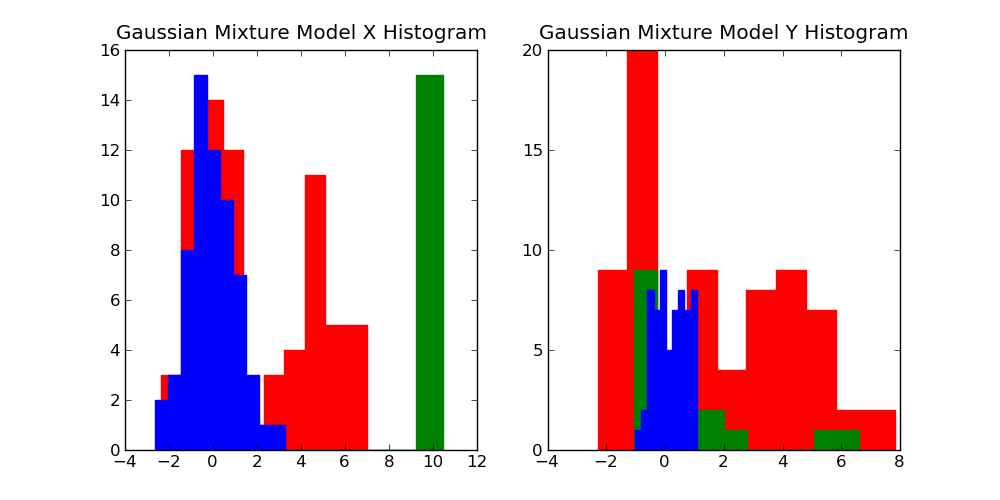
\includegraphics[width=18cm]{GMMhist.png}
\caption{Histogram of Gaussian Mixture Model}
\label{gmmhist}
\end{figure}

\end{itemize}

\end{document}